\chapter{Plotting with Tikz (Part II)}

\paragraph{Introduction}
This chapter continues to discuss the finer details and broad applications of TikZ plotting.

\section{Advanced Axis Control}

\subsection{Axis Scales}

\paragraph{Axis Units}
We can adjust the units of the coordinate axes in a TikZ plot by specifying them at the beginning. This is readily demonstrated in the small example of Figure \ref{fig:newcoord1} below.
\begin{lstlisting}
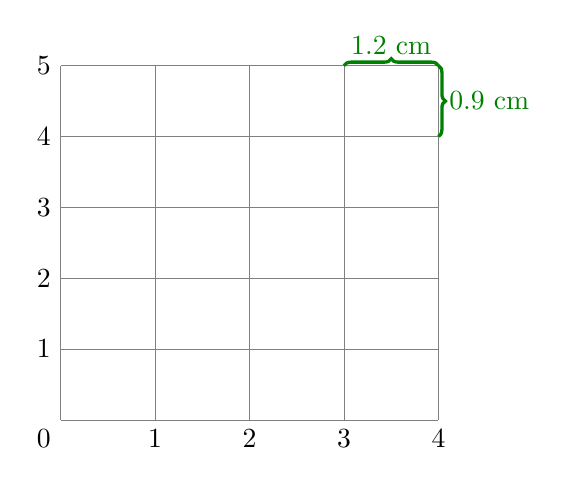
\begin{tikzpicture}[x=1.2cm, y=0.9cm]
\draw[help lines, step = {(1,1)}] (0,0) grid (4,5);
\node at (0,0) [below left] {$0$};
\foreach \ii in {1,...,4} {\node at (\ii,0) [below]{$\ii$};}
\foreach \jj in {1,...,5} {\node at (0,\jj) [left]{$\jj$};}
\draw[decorate, decoration=brace, very thick, Green] (3,5) -- (4,5) node [midway, above] {$1.2$ cm}; 
\draw[decorate, decoration={brace, mirror}, very thick, Green] (4,4) -- (4,5) node [midway, right] {$0.9$ cm};
\end{tikzpicture}    
\end{lstlisting}
\begin{figure}
    \centering
    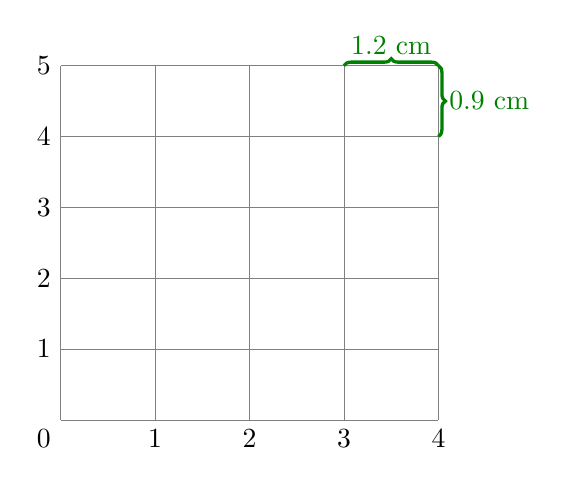
\begin{tikzpicture}[x=1.2cm, y=0.9cm]
    \draw[help lines, step = {(1,1)}] (0,0) grid (4,5);
    \node at (0,0) [below left] {$0$};
    \foreach \ii in {1,...,4} {\node at (\ii,0) [below]{$\ii$};}
    \foreach \jj in {1,...,5} {\node at (0,\jj) [left]{$\jj$};}
    \draw[decorate, decoration=brace, very thick, Green] (3,5) -- (4,5) node [midway, above] {$1.2$ cm}; 
    \draw[decorate, decoration={brace, mirror}, very thick, Green] (4,4) -- (4,5) node [midway, right] {$0.9$ cm};
    \end{tikzpicture}
    \caption{Cartesian coordinate system transformation.}
    \label{fig:newcoord1}
\end{figure}
Be reminded that after the scale transformation, we have to supply \texttt{step = {(1,1)}} so that the grid lines are drawn in the new units. We have also used the \texttt{brace} and \texttt{mirror} decorations, which are not hard to understand.

\paragraph{Coordinate Rotation}
Another simple way to transform the coordinate axes is via rotation. It is extremely straightforward and immediately done in Figure \ref{fig:newcoord2}.
\begin{lstlisting}

\begin{tikzpicture}[x=1.2cm, y=0.9cm, rotate=20]
\draw[help lines, step = {(1,1)}] (0,0) grid (4,5);
\end{tikzpicture}       
\end{lstlisting}
\begin{figure}
    \centering
    
\begin{tikzpicture}[x=1.2cm, y=0.9cm, rotate=20]
    \draw[help lines, step = {(1,1)}] (0,0) grid (4,5);
    \end{tikzpicture}
    \caption{Same as Figure \ref{fig:newcoord1} but with an anti-clockwise rotation applied to the frame.}
    \label{fig:newcoord2}
\end{figure}

\subsection{3D Plotting}

\paragraph{3D Coordinate Axes}
To initiate a 3D TikZ plot, the easiest automatic way is to write the drawing code just as usual, but now with the coordinates being 3D. We can also control the axis scales, like in the 2D scenario, where we can specify the direction of each axis displayed on the page. This is demonstrated in Figure \ref{fig:3dvec}.
\begin{lstlisting}
\begin{tikzpicture}[x={(-1cm, -1.5cm)}, y={(1.5cm, -0.75cm)}, z={(0cm, 1.8cm)}, every path/.append style={>=Latex}]
\draw [->] (0,0,0) -- (3,0,0) node [below left] {$x$};
\draw [->] (0,0,0) -- (0,3,0) node [below right] {$y$};
\draw [->] (0,0,0) -- (0,0,3) node [above] {$z$};
\draw [->, very thick, Red] (0,0,0) -- (1,0,0) node [left] {$\hat{\imath} = (1,0,0)^T$};
\draw [->, very thick, Red] (0,0,0) -- (0,1,0) node [above right, midway] {$\hat{\jmath} = (0,1,0)^T$} ; 
\draw [->, very thick, Red] (0,0,0) -- (0,0,1) node [left] {$\hat{k} = (0,0,1)^T$};
\draw [Gray, dashed] (1,2,0) -- (1,0,0) node[below, midway, sloped]{$y=2$}; 
\draw [Gray, dashed] (1,2,0) -- (0,2,0) node[below, midway, sloped]{$x=1$}; 
\draw [Gray, dashed] (1,2,0) -- (1,2,2.5) node[midway, right]{$z=2.5$};
\draw [->, blue, line width=1.2] (0,0,0) -- (1,2,2.5) node [right] {$\vec{v} = (1,2,2.5)^T$};
\end{tikzpicture}    
\end{lstlisting}
\begin{figure}[ht!]
    \centering
    \begin{tikzpicture}[x={(-1cm, -1.5cm)}, y={(1.5cm, -0.75cm)}, z={(0cm, 1.8cm)}, every path/.append style={>=Latex}]
    \draw [->] (0,0,0) -- (2,0,0) node [below left] {$x$};
    \draw [->] (0,0,0) -- (0,2,0) node [below right] {$y$};
    \draw [->] (0,0,0) -- (0,0,2) node [above] {$z$};
    \draw [->, very thick, Red] (0,0,0) -- (1,0,0) node [left] {$\hat{\imath} = (1,0,0)^T$};
    \draw [->, very thick, Red] (0,0,0) -- (0,1,0) node [above right, midway] {$\hat{\jmath} = (0,1,0)^T$} ; 
    \draw [->, very thick, Red] (0,0,0) -- (0,0,1) node [left] {$\hat{k} = (0,0,1)^T$};
    \draw [Gray, dashed] (1,2,0) -- (1,0,0) node[below, midway, sloped]{$y=2$}; 
    \draw [Gray, dashed] (1,2,0) -- (0,2,0) node[below, midway, sloped]{$x=1$}; 
    \draw [Gray, dashed] (1,2,0) -- (1,2,2.5) node[midway, right]{$z=2.5$};
    \draw [->, blue, line width=1.2] (0,0,0) -- (1,2,2.5) node [right] {$\vec{v} = (1,2,2.5)^T$};
    \end{tikzpicture}
    \caption{A vector in three-dimensional space.}
    \label{fig:3dvec}
\end{figure}
Notice that we have utilized the \texttt{append style} function to add the requirement that all arrow tips will use the \texttt{LaTeX} type.

\paragraph{Surface Plots}
Moving from 2D to 3D, we may now want to draw surface plots instead of just curves. This can be done by declaring a normal axis scope and using the \texttt{\textbackslash addplot3} command with the \texttt{surf} keyword on the level equation. Figure \ref{fig:2dgauss} below serves as an example.
\begin{lstlisting}
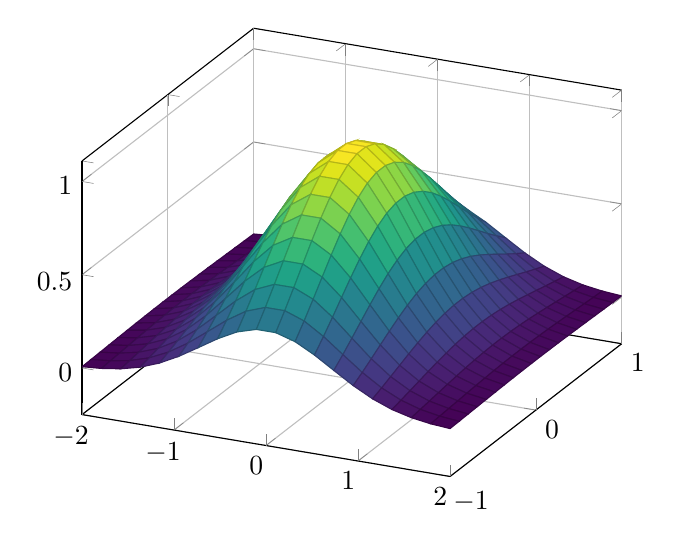
\begin{tikzpicture}
\begin{axis}[grid=major,colormap/viridis,zmin=-0.25]
\addplot3[surf,samples=20,domain=-2:2,y domain=-1:1] {exp(-(x^2+y^2))};
\end{axis}
\end{tikzpicture}    
\end{lstlisting}
\begin{figure}
    \centering
    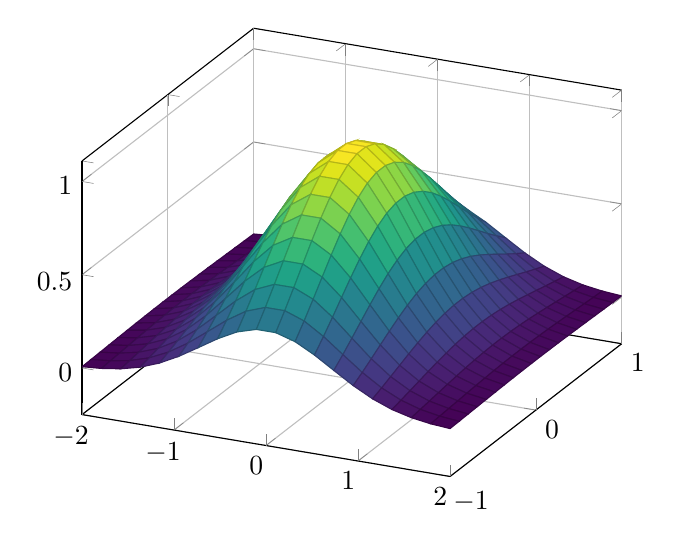
\begin{tikzpicture}
    \begin{axis}[grid=major,colormap/viridis,zmin=-0.25]
    \addplot3[surf,samples=20,domain=-2:2,y domain=-1:1] {exp(-(x^2+y^2))};
    \end{axis}
    \end{tikzpicture}
    \caption{A 2D Gaussian surface plot.}
    \label{fig:2dgauss}
\end{figure}
We can add a mesh grid and choose the color map (viridis here) at the start of the axis environment. It is also possible to provide a \texttt{colorbar}. To draw a contour plot instead, we simply replace \texttt{surf} by \texttt{contour gnuplot}\footnote{Or \texttt{contour lua} if you are using LuaLaTeX.} and use the \texttt{view=\{0\}\{90\}} trick introduced at the end of the last chapter.

\paragraph{3D Spheres and Arcs}
To construct a 3D sphere and draw arcs on it, we need to import the \texttt{tikz-3dplot} package (requires \texttt{\textbackslash usepackage\{tikz-3dplot\}} \footnote{A positive side effect is that it also loads the smaller \texttt{3d} TikZ library, which allows the user to write in cylindrical/spherical coordinates.} this time).  Drawing only the sphere is not hard (plus the \texttt{ball color} option). Meanwhile, drawing the arcs requires us to first locate the center as well as the two ends of each of them via \texttt{\textbackslash tdplotdefinepoints}, and then actually execute that with \texttt{\textbackslash tdplotdrawpolytopearc}. The whole procedure is illustrated by Figure \ref{fig:spherearc}.
\begin{lstlisting}
\tdplotsetmaincoords{70}{110}
\begin{tikzpicture}[scale=2.5,tdplot_main_coords,rotate=15]
\coordinate (O) at (0,0,0);
\draw [ball color=white,very thin] (O) circle (1cm);
\tdplotdefinepoints(0,0,0)(0,0,1)(3^0.5/2,0,0.5)
\tdplotdrawpolytopearc[thick, red]{1}{left, red}{$a$}
\tdplotdefinepoints(0,0,0)(0,0,1)(0,0.8,0.6)
\tdplotdrawpolytopearc[thick, blue]{1}{above, blue}{$b$}
\tdplotdefinepoints(0,0,0)(0,0.8,0.6)(3^0.5/2,0,0.5)
\tdplotdrawpolytopearc[thick, Green]{1}{below, Green}{$c$}
\draw[dashed, color=black!60] (O) -- (0,0,1) node(C){};
\draw[dashed, color=black!60] (O) -- (3^0.5/2,0,0.5) node(B){};
\draw[dashed, color=black!60] (O) -- (0,0.8,0.6) node(A){};
\end{tikzpicture}    
\end{lstlisting}
\begin{figure}
    \centering
    \tdplotsetmaincoords{70}{110}
    \begin{tikzpicture}[scale=2.5,tdplot_main_coords,rotate=15]
    \coordinate (O) at (0,0,0);
    \draw [ball color=white,very thin] (O) circle (1cm);
    \tdplotdefinepoints(0,0,0)(0,0,1)(3^0.5/2,0,0.5)
    \tdplotdrawpolytopearc[thick, red]{1}{left, red}{$a$}
    \tdplotdefinepoints(0,0,0)(0,0,1)(0,0.8,0.6)
    \tdplotdrawpolytopearc[thick, blue]{1}{above, blue}{$b$}
    \tdplotdefinepoints(0,0,0)(0,0.8,0.6)(3^0.5/2,0,0.5)
    \tdplotdrawpolytopearc[thick, Green]{1}{below, Green}{$c$}
    \draw[dashed, color=black!60] (O) -- (0,0,1) node(C){};
    \draw[dashed, color=black!60] (O) -- (3^0.5/2,0,0.5) node(B){};
    \draw[dashed, color=black!60] (O) -- (0,0.8,0.6) node(A){};
    \end{tikzpicture}    
    \caption{Drawing a sphere with a spherical triangle on it.}
    \label{fig:spherearc}
\end{figure}
Note that we also call \texttt{\textbackslash tdplotsetmaincoords} and deploy \texttt{tdplot\_main\_\allowbreak coords} to adjust the viewing angle. Furthermore, we have used the \texttt{rotate} option as a workaround to tune the orientation.

\section{Data Visualization}

\paragraph{Line Charts}
There are many other types of plots that we can make with TikZ. The most basic one will probably be line charts, and we will use the Mauna Loa $\text{CO}_2$ concentration data (downloaded from \href{https://gml.noaa.gov/webdata/ccgg/trends/co2/co2_annmean_mlo.csv}{https://gml.noaa.gov/webdata/ccgg/trends/co2/\allowbreak co2\_annmean\_mlo.csv}) as an example. As before, the \texttt{\textbackslash addplot} command is called, and it can accept and read a \texttt{.csv} (comma-separated values) file. We will supply the one downloaded from the link above, while providing the respective header names for the \texttt{x} and \texttt{y} axes. The result is shown in Figure \ref{fig:CO2} above.
\begin{lstlisting}
\begin{tikzpicture}
\begin{axis}[width=0.95\textwidth, height=0.65\textwidth, x tick label style={rotate=45,/pgf/number format/.cd,set thousands separator={}}, enlarge x limits={abs=2}, xlabel=year, ylabel=$\text{CO}_2$ concentration (ppm), title=Mauna Loa Observatory Measurement, xlabel style={yshift=-15pt}]
\addplot[Green, mark=*] table [x=year, y=mean, col sep=comma] {co2_annmean_mlo.csv};
\end{axis}
\end{tikzpicture}    
\end{lstlisting}
\begin{figure}
    \centering
    \begin{tikzpicture}
    \begin{axis}[width=0.95\textwidth, height=0.65\textwidth, x tick label style={rotate=45,/pgf/number format/.cd,set thousands separator={}}, enlarge x limits={abs=2}, xlabel=year, ylabel=$\text{CO}_2$ concentration (ppm), title=Mauna Loa Observatory Measurement, xlabel style={yshift=-15pt}]
    \addplot[Green, mark=*] table [x=year, y=mean, col sep=comma] {co2_annmean_mlo.csv};
    \end{axis}
    \end{tikzpicture}
    \caption{The time-series of $\text{CO}_2$ concentration recorded at Mauna Loa Observatory from 1959 to 2024.}
    \label{fig:CO2}
\end{figure}
Some noticeable points include that if we change the graph color, we have to explicitly append \texttt{mark=*} to get back the dot marks along the curve. Removing it will produce only the curve. We enforce \texttt{enlarge x limits} to take \texttt{abs=2} so that the $x$-domain extends by $2$ years. We also rotate the $x$-axis ticks by $45^\circ$ and use some options to format out the \texttt{,} originally in the year numbers. (Try removing them to see what happens!) Accounting for that, we also shift the $x$-axis label downward by $15$ pt.

\paragraph{Bar Plots}
Bar plots are another commonly seen plot type. To construct a bar plot, we either declare \texttt{xbar} or \texttt{ybar} in the \texttt{axis} option at the start and call the \texttt{\textbackslash addplot} command for each set of bars, or put the keyword directly after \texttt{\textbackslash addplot}. A small example is given as Figure \ref{fig:classscore}.
\begin{lstlisting}
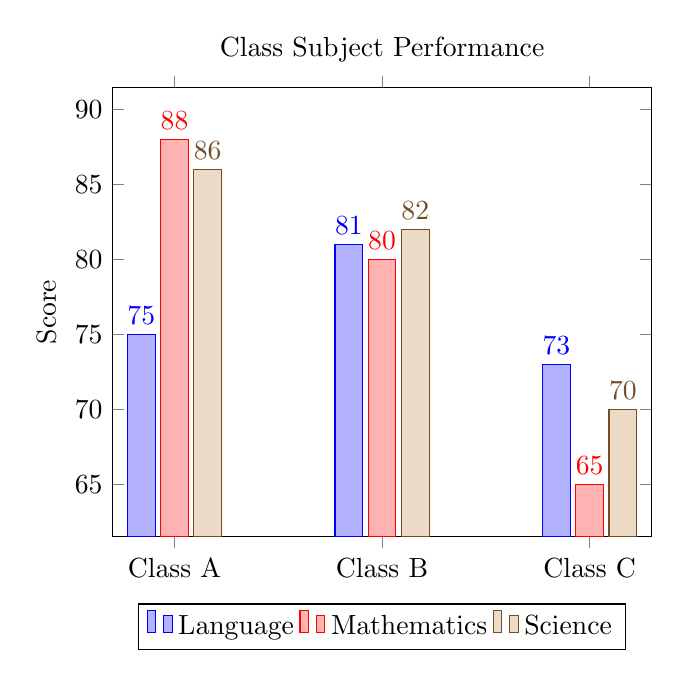
\begin{tikzpicture}
\begin{axis}[title=Class Subject Performance,
    ybar,
    enlargelimits=0.15,
    legend style={at={(0.5,-0.15)},anchor=north,legend columns=-1},
    ylabel=Score,
    symbolic x coords={Class A,Class B,Class C},
    xtick=data, 
    nodes near coords,
    nodes near coords align=vertical]
\addplot coordinates {(Class A,75) (Class B,81) (Class C,73)};
\addplot coordinates {(Class A,88) (Class B,80) (Class C,65)};
\addplot coordinates {(Class A,86) (Class B,82) (Class C,70)};
\legend{Language,Mathematics,Science}
\end{axis}
\end{tikzpicture}
\end{lstlisting}
\begin{figure}
    \centering
    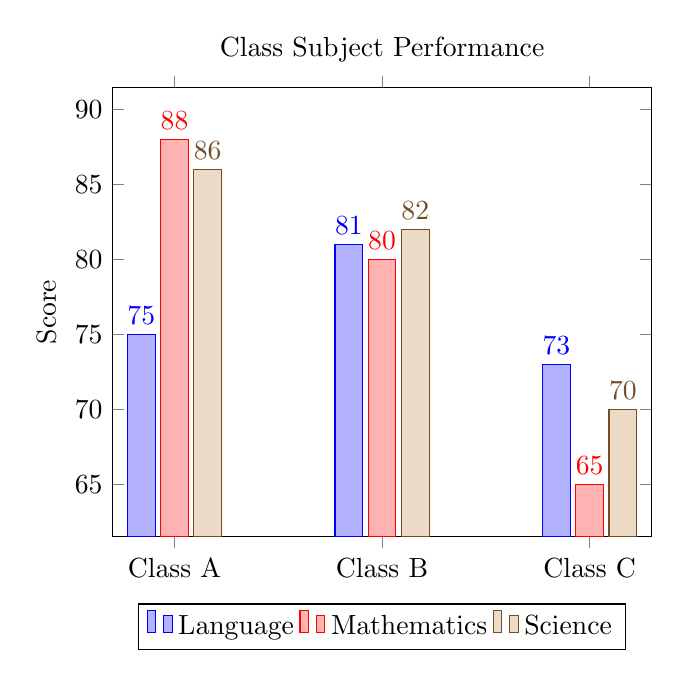
\begin{tikzpicture}
    \begin{axis}[title=Class Subject Performance,
    ybar,
    enlargelimits=0.15,
    legend style={at={(0.5,-0.15)},anchor=north,legend columns=-1},
    ylabel=Score,
    symbolic x coords={Class A,Class B,Class C},
    xtick=data, 
    nodes near coords,
    nodes near coords align=vertical]
    \addplot coordinates {(Class A,75) (Class B,81) (Class C,73)};
    \addplot coordinates {(Class A,88) (Class B,80) (Class C,65)};
    \addplot coordinates {(Class A,86) (Class B,82) (Class C,70)};
    \legend{Language,Mathematics,Science}
    \end{axis}
    \end{tikzpicture}
    \caption{A toy dataset about the scores of three classes in three different subjects.}
    \label{fig:classscore}
\end{figure}
Here we use \texttt{symbolic x coords} to tell the \texttt{axis} that the $x$-coordinates should be treated as strings, and \texttt{xtick=data} guarantees that the ticks will be as the input data. \texttt{nodes near coords} produces the numbers above the bars. Last but not least, we have tweaked the style for the legend, particularly \texttt{legend columns=-1} to arrange the entries horizontally.

\section{Referencing between TikZ Pictures}

\paragraph{Remembering Names and Overlay}
Sometimes we need to combine multiple TikZ pictures, and share name labels between them so that they can refer to objects in each other. We can enable this functionality by setting the \texttt{remember picture} option for them. This is demonstrated by the rather lengthy example of different phase portraits in Figure \ref{fig:phasediagram}.
\begin{lstlisting}
\tikzset{decorated arrows/.style={postaction=decorate,
         decoration={markings,mark={at position 0.5 with {\arrow{stealth}}}}}}
% Main Classifying Diagram
\begin{tikzpicture}[remember picture]
\draw[thick, ->] (-6,0) -- (6,0) node[right]{$\tr(A)$};
\draw[thick, ->] (0,-6) -- (0,6) node[above]{$\det(A)$};
\node[below left] (O) at (0,0) {$O$}; 
\draw[gray, thick] plot[domain=-4.5:4.5,samples=100] (\x, {(\x)^2/4});
\node[gray, rotate=-60] at (-3.5,2.5) {$\Delta = \tr(A)^2 - 4\det(A) = 0$};
\node[gray, rotate=60] at (3,3) {Complex};
\node[gray, rotate=60] at (3.5,2.5) {Real};
\node[anchor=center, Green, rotate=90] at (-6, 5) {\large Stable};
\node[anchor=center, Red, rotate=-90] at (6, 5) {\large Unstable};
% Defining the named coordinates
\coordinate (saddle) at (0,-3);
\node[anchor=center, blue] at (0,-5) {Saddle Point};
\coordinate (center) at (0,3);
\node[anchor=center, blue] at (0, 1) {Center};
... % omitted other cases
\end{tikzpicture} 
% Saddle Point
\begin{tikzpicture}[remember picture, overlay]
\begin{axis}[at=(saddle), anchor=center, scale=0.5, xmin=-2, xmax=2, ymin=-2, ymax=2, axis lines=center, hide axis]
\addplot[domain=-1:1.5,samples=50,blue,decorated arrows] ({0.5*e^(x) + 0.5*e^(-x)},{0.5*e^(x) - 1*e^(-x)});
\addplot[domain=-1.5:2,samples=50,blue,decorated arrows] ({0.3*e^(x) + 0.3*e^(-x)},{0.3*e^(x) - 0.6*e^(-x)});
\addplot[domain=-1:1.5,samples=50,blue,decorated arrows] ({0.5*e^(x) - 0.5*e^(-x)},{0.5*e^(x) + 1*e^(-x)});
\addplot[domain=-1.5:2,samples=50,blue,decorated arrows] ({0.3*e^(x) - 0.3*e^(-x)},{0.3*e^(x) + 0.6*e^(-x)});
...
\end{axis}
\end{tikzpicture}
% Center
\begin{tikzpicture}[remember picture, overlay]
\begin{axis}[at=(center), anchor=center, scale=0.5, xmin=-2, xmax=2, ymin=-2, ymax=2, axis lines=center, hide axis]
\addplot[domain=0:360,samples=50,blue,decorated arrows] ({1*(cos(x)) + 0.8*(sin(x))},{-1*(cos(x)) + 1*(sin(x))});
\addplot[domain=0:360,samples=50,blue,decorated arrows] ({2/3*(cos(x)) + 1.6/3*(sin(x))},{-2/3*(cos(x)) + 2/3*(sin(x))});
\addplot[domain=0:360,samples=50,blue,decorated arrows] ({1/3*(cos(x)) + 0.8/3*(sin(x))},{-1/3*(cos(x)) + 1/3*(sin(x))});
\end{axis}
\end{tikzpicture}
...
\end{lstlisting}
\tikzset{decorated arrows/.style={postaction=decorate,
        decoration={markings,mark={at position 0.5 with {\arrow{stealth}}}}}}
\begin{figure}
    \centering
    \begin{tikzpicture}[remember picture]
    \draw[thick, ->] (-6,0) -- (6,0) node[right]{$\tr(A)$};
    \draw[thick, ->] (0,-6) -- (0,6) node[above]{$\det(A)$};
    \node[below left] (O) at (0,0) {$O$}; 
    \draw[gray, thick] plot[domain=-4.5:4.5,samples=100] (\x, {(\x)^2/4});
    \node[gray, rotate=-60] at (-3.5,2.5) {$\Delta = \tr(A)^2 - 4\det(A) = 0$};
    \node[gray, rotate=60] at (3,3) {Complex};
    \node[gray, rotate=60] at (3.5,2.5) {Real};
    \node[anchor=center, Green, rotate=90] at (-6, 5) {\large Stable};
    \node[anchor=center, Red, rotate=-90] at (6, 5) {\large Unstable};
    \coordinate (saddle) at (0,-3);
    \node[anchor=center, blue] at (0,-5) {Saddle Point};
    \coordinate (center) at (0,3);
    \node[anchor=center, blue] at (0, 1) {Center};
    \coordinate (stablespir) at (-3, 6);
    \node[anchor=center, blue] at (-3, 8) {Stable Spiral};
    \coordinate (unstablespir) at (3, 6);
    \node[anchor=center, blue] at (3, 8) {Unstable Spiral};
    \coordinate (sink) at (-5, 1);
    \node[anchor=center, blue] at (-5.5, 3) {Sink};
    \coordinate (source) at (5, 1);
    \node[anchor=center, blue] at (5.5, 3) {Source};
    \end{tikzpicture}
    \begin{tikzpicture}[remember picture, overlay]
    \begin{axis}[at=(saddle), anchor=center, scale=0.5, xmin=-2, xmax=2, ymin=-2, ymax=2,
    axis lines=center, hide axis]
    \addplot[domain=-1:1.5,samples=50,blue,decorated arrows] ({0.5*e^(x) + 0.5*e^(-x)},{0.5*e^(x) - 1*e^(-x)});
    \addplot[domain=-1.5:2,samples=50,blue,decorated arrows] ({0.3*e^(x) + 0.3*e^(-x)},{0.3*e^(x) - 0.6*e^(-x)});
    \addplot[domain=-1:1.5,samples=50,blue,decorated arrows] ({0.5*e^(x) - 0.5*e^(-x)},{0.5*e^(x) + 1*e^(-x)});
    \addplot[domain=-1.5:2,samples=50,blue,decorated arrows] ({0.3*e^(x) - 0.3*e^(-x)},{0.3*e^(x) + 0.6*e^(-x)});
    \addplot[domain=-1:1.5,samples=50,blue,decorated arrows] ({-(0.5*e^(x) + 0.5*e^(-x))},{-(0.5*e^(x) - 1*e^(-x))});
    \addplot[domain=-1.5:2,samples=50,blue,decorated arrows] ({-(0.3*e^(x) + 0.3*e^(-x))},{-(0.3*e^(x) - 0.6*e^(-x))});
    \addplot[domain=-1:1.5,samples=50,blue,decorated arrows] ({-(0.5*e^(x) - 0.5*e^(-x))},{-(0.5*e^(x) + 1*e^(-x))});
    \addplot[domain=-1.5:2,samples=50,blue,decorated arrows] ({-(0.3*e^(x) - 0.3*e^(-x))},{-(0.3*e^(x) + 0.6*e^(-x))});
    \addplot[domain=0:2,samples=50,blue,decorated arrows] ({-x},{-x});
    \addplot[domain=0:2,samples=50,blue,decorated arrows] ({x},{x});
    \addplot[domain=0:2,samples=50,blue,decorated arrows] ({-0.5*(2-x)},{(2-x)});
    \addplot[domain=0:2,samples=50,blue,decorated arrows] ({0.5*(2-x)},{-(2-x)});
    \end{axis}
    \end{tikzpicture}
    \begin{tikzpicture}[remember picture, overlay]
    \begin{axis}[at=(center), anchor=center, scale=0.5, xmin=-2, xmax=2, ymin=-2, ymax=2,
    axis lines=center, hide axis]
    \addplot[domain=0:360,samples=50,blue,decorated arrows] ({1*(cos(x)) + 0.8*(sin(x))},{-1*(cos(x)) + 1*(sin(x))});
    \addplot[domain=0:360,samples=50,blue,decorated arrows] ({2/3*(cos(x)) + 1.6/3*(sin(x))},{-2/3*(cos(x)) + 2/3*(sin(x))});
    \addplot[domain=0:360,samples=50,blue,decorated arrows] ({1/3*(cos(x)) + 0.8/3*(sin(x))},{-1/3*(cos(x)) + 1/3*(sin(x))});
    \end{axis}
    \end{tikzpicture}
    \begin{tikzpicture}[remember picture, overlay]
    \begin{axis}[at=(stablespir), anchor=center, scale=0.5, xmin=-2, xmax=2, ymin=-2, ymax=2,
    axis lines=center, hide axis]
    \addplot[domain=0:1.99,samples=200,blue,decorated arrows] ({1*(2-x)*(sin(2*deg(ln(2-x))) - 0.5*(2-x)*(cos(2*deg(ln(2-x)))},{1*(2-x)*(cos(2*deg(ln(2-x))) + 0.5*(2-x)*(sin(2*deg(ln(2-x)))});
    \addplot[domain=0:1.99,samples=200,blue,decorated arrows] ({-1*(2-x)*(sin(2*deg(ln(2-x))) + 0.5*(2-x)*(cos(2*deg(ln(2-x)))},{-1*(2-x)*(cos(2*deg(ln(2-x))) - 0.5*(2-x)*(sin(2*deg(ln(2-x)))});
    \addplot[domain=0:1.99,samples=200,blue,decorated arrows] ({1*(2-x)*(sin(2*deg(ln(2-x))) + 0.5*(2-x)*(cos(2*deg(ln(2-x)))},{1*(2-x)*(cos(2*deg(ln(2-x))) - 0.5*(2-x)*(sin(2*deg(ln(2-x)))});
    \addplot[domain=0:1.99,samples=200,blue,decorated arrows] ({-1*(2-x)*(sin(2*deg(ln(2-x))) - 0.5*(2-x)*(cos(2*deg(ln(2-x)))},{-1*(2-x)*(cos(2*deg(ln(2-x))) + 0.5*(2-x)*(sin(2*deg(ln(2-x)))});
    \end{axis}
    \end{tikzpicture}
    \begin{tikzpicture}[remember picture, overlay]
    \begin{axis}[at=(unstablespir), anchor=center, scale=0.5, xmin=-2, xmax=2, ymin=-2, ymax=2,
    axis lines=center, hide axis]
    \addplot[domain=0.01:2,samples=200,blue,decorated arrows] ({1*x*(cos(2*deg(ln(x)))},{0.8*(x)*(sin(2*deg(ln(x)))});
    \addplot[domain=0.01:2,samples=200,blue,decorated arrows] ({-1*x*(cos(2*deg(ln(x)))},{-0.8*(x)*(sin(2*deg(ln(x)))});
    \end{axis}
    \end{tikzpicture}
    \begin{tikzpicture}[remember picture, overlay]
    \begin{axis}[at=(sink), anchor=center, scale=0.5, xmin=-2, xmax=2, ymin=-2, ymax=2,
    axis lines=center, hide axis]
    \addplot[domain=0:1.5,samples=200,blue,decorated arrows] ({0.6*(1.5-x) + 0.6*(1.5-x)^2},{-0.6*(1.5-x) + 0.6*(1.5-x)^2});
    \addplot[domain=0:1.5,samples=200,blue,decorated arrows] ({1*(1.5-x) + 0.2*(1.5-x)^2},{-1*(1.5-x) + 0.2*(1.5-x)^2});
    \addplot[domain=0:1.5,samples=200,blue,decorated arrows] ({-0.6*(1.5-x) + 0.6*(1.5-x)^2},{0.6*(1.5-x) + 0.6*(1.5-x)^2});
    \addplot[domain=0:1.5,samples=200,blue,decorated arrows] ({-1*(1.5-x) + 0.2*(1.5-x)^2},{1*(1.5-x) + 0.2*(1.5-x)^2});
    \addplot[domain=0:1.5,samples=200,blue,decorated arrows] ({-(0.6*(1.5-x) + 0.6*(1.5-x)^2)},{-(-0.6*(1.5-x) + 0.6*(1.5-x)^2)});
    \addplot[domain=0:1.5,samples=200,blue,decorated arrows] ({-(1*(1.5-x) + 0.2*(1.5-x)^2)},{-(-1*(1.5-x) + 0.2*(1.5-x)^2)});
    \addplot[domain=0:1.5,samples=200,blue,decorated arrows] ({-(-0.6*(1.5-x) + 0.6*(1.5-x)^2)},{-(0.6*(1.5-x) + 0.6*(1.5-x)^2)});
    \addplot[domain=0:1.5,samples=200,blue,decorated arrows] ({-(-1*(1.5-x) + 0.2*(1.5-x)^2)},{-(1*(1.5-x) + 0.2*(1.5-x)^2)});
    \addplot[domain=0:1.5,samples=100,blue,decorated arrows]({1*(1.5-x)},{-1*(1.5-x)});
    \addplot[domain=0:1.5,samples=100,blue,decorated arrows]({-1*(1.5-x)},{1*(1.5-x)});
    \addplot[domain=0:1.5,samples=100,blue,decorated arrows]({0.6*(1.5-x)^2},{0.6*(1.5-x)^2});
    \addplot[domain=0:1.5,samples=100,blue,decorated arrows]({-0.6*(1.5-x)^2},{-0.6*(1.5-x)^2});
    \end{axis}
    \end{tikzpicture}
    \begin{tikzpicture}[remember picture, overlay]
    \begin{axis}[at=(source), anchor=center, scale=0.5, xmin=-2, xmax=2, ymin=-2, ymax=2,
    axis lines=center, hide axis]
    \addplot[domain=0:1.5,samples=200,blue,decorated arrows] ({0.8*x^1.5 + 0.2*x},{-0.4*x^1.5 + 0.6*x});
    \addplot[domain=0:1.5,samples=200,blue,decorated arrows] ({-0.8*x^1.5 + 0.2*x},{0.4*x^1.5 + 0.6*x});
    \addplot[domain=0:1.5,samples=200,blue,decorated arrows] ({-(0.8*x^1.5 + 0.2*x)},{-(-0.4*x^1.5 + 0.6*x)});
    \addplot[domain=0:1.5,samples=200,blue,decorated arrows] ({-(-0.8*x^1.5 + 0.2*x)},{-(0.4*x^1.5 + 0.6*x)});
    \addplot[domain=0:1.5,samples=200,blue,decorated arrows] ({-1.2*x^1.5},{0.6*x^1.5});
    \addplot[domain=0:1.5,samples=200,blue,decorated arrows] ({1.2*x^1.5},{-0.6*x^1.5});
    \addplot[domain=0:1.5,samples=200,blue,decorated arrows] ({0.3*x},{0.9*x});
    \addplot[domain=0:1.5,samples=200,blue,decorated arrows] ({-0.3*x},{-0.9*x});
    \end{axis}
    \end{tikzpicture}
    \caption{Different types of equilibrium points and their representative phase portraits in two-dimensional dynamical systems.}
    \label{fig:phasediagram}
\end{figure}
(The full code can be checked from the source file.) In the main procedure, the underlying axes and parabola are drawn, and the coordinates at which each phase portrait will be placed are marked and named. Then, a smaller TikZ picture is initiated for each type over the main diagram with the \texttt{overlay} option. The axis containing the phase lines is then centered at the marked coordinates by filling the \texttt{at} option with the shared name.

\section{Matrices in Tikz}

\paragraph{Matrices of Nodes}
To generate a matrix in TikZ that can be marked, we can use the \texttt{\textbackslash matrix} command with the \texttt{matrix of math nodes} option. This is illustrated by Figure \ref{fig:tikzmatrix} below.
\begin{lstlisting}
\begin{tikzpicture}[remember picture]
\node (A) {$A=$};
\matrix(mymatrix)[matrix of math nodes, left delimiter={[}, right delimiter={]}, right=1.5ex of A, row sep=6pt, column sep=6pt, inner sep=1.5pt, nodes={text width=16pt, align=center}]
{2 & 1 & 7 & \frac{8}{9} \\
\mathcolor{red}{5} & -\frac{1}{3} & 5 & 0 \\
-3 & \frac{4}{11} & 6 & -\frac{1}{6} \\};
\begin{scope}[on background layer]
\draw [Green, dashed, fill=blue!12, fill opacity=0.5] ($(mymatrix-1-1.north west)+(-0.5ex,1ex)$) rectangle ($(mymatrix-3-1.south east)+(0.5ex,-1ex)$);
\draw [Green, dashed, fill=blue!12, fill opacity=0.5] ($(mymatrix-2-1.north west)+(-0.5ex,1ex)$) rectangle ($(mymatrix-2-4.south east)+(0.5ex,-1ex)$);
\end{scope}
\node at (mymatrix-1-1) [above, font=\footnotesize, yshift=10, Green] {Col 1};
\node at (mymatrix-2-4) [right, font=\footnotesize, xshift=15, Green] {Row 2};
\draw[Red, -Stealth] (pic cs:Ap) to[in=-45, out=-180] (mymatrix-2-1);
\end{tikzpicture}
{\large$\mathcolor{red}{\tikzmark{Ap}A_{21} = 5}$}    
\end{lstlisting}
\begin{figure}
    \centering
    \begin{tikzpicture}[remember picture]
    \node (A) {$A=$};
    \matrix(mymatrix)[matrix of math nodes, left delimiter={[}, 
    right delimiter={]}, right=1.5ex of A, row sep=6pt,
    column sep=6pt, inner sep=1.5pt, nodes={text width=16pt, align=center}]
    {2 & 1 & 7 & \frac{8}{9} \\
    \mathcolor{red}{5} & -\frac{1}{3} & 5 & 0 \\
    -3 & \frac{4}{11} & 6 & -\frac{1}{6} \\};
    \begin{scope}[on background layer]
    \draw [Green, dashed, fill=blue!12, fill opacity=0.5] ($(mymatrix-1-1.north west)+(-0.5ex,1ex)$) rectangle ($(mymatrix-3-1.south east)+(0.5ex,-1ex)$);
    \draw [Green, dashed, fill=blue!12, fill opacity=0.5] ($(mymatrix-2-1.north west)+(-0.5ex,1ex)$) rectangle ($(mymatrix-2-4.south east)+(0.5ex,-1ex)$);
    \end{scope}
    \node at (mymatrix-1-1) [above, font=\footnotesize, yshift=10, Green] {Col 1};
    \node at (mymatrix-2-4) [right, font=\footnotesize, xshift=15, Green] {Row 2};
    \draw[Red, -Stealth] (pic cs:Ap) to[in=-45, out=-180] (mymatrix-2-1);
    \end{tikzpicture}
    {\large$\mathcolor{red}{\tikzmark{Ap}A_{21} = 5}$}
    \caption{Typesetting and labeling a TikZ matrix.}
    \label{fig:tikzmatrix}
\end{figure}
Particularly, the \texttt{left/right delimiter} settings enclose the nodes with the square brackets, and the \texttt{right of} syntax puts the matrix to the right of the \texttt{A=} part. The positioning of the nodes can be controlled by changing \texttt{row sep}, \texttt{column sep}, and \texttt{inner sep}. 

We have also used two additional TikZ libraries. The first one is \texttt{backgrounds} to draw blue shadings along the targeted row/column in the background via a \texttt{on background layer} scope. The second one is \texttt{tikzmark} so that we can place a corresponding \texttt{tikzmark} tag at some other location outside the TikZ picture, which can then refer to this tag as \texttt{pic cs:<name>} with the help of \texttt{remember picture} just introduced before.

\section{Flow Charts}

\paragraph{Flow Charts with Shapes}
A general TikZ application is to produce flow charts for various processes. This is demonstrated by the bisection algorithm example in Figure \ref{fig:bisect}. We will need to load the \texttt{shapes.geometric} TikZ library for the shapes representing different components.
\begin{lstlisting}
\begin{tikzpicture}[startend/.style={rectangle, rounded corners, minimum width=3cm, minimum height=1cm, draw=black},
io/.style={trapezium, trapezium left angle=70, trapezium right angle=110, minimum width=4cm, minimum height=1cm, draw=black},
process/.style={rectangle, minimum width=3cm, minimum height=1cm, draw=black},
decision/.style={diamond, minimum width=5cm, minimum height=1cm, draw=black}]
\node[startend] (start) {Start};
\node[io,below=1.2cm of start,align=center] (input) {$f(x)$, $a < b$, \\ $f(a)<0$, $f(b)>0$};
\draw[->] (start) -- (input);
\node[process,below=1.2cm of input] (bisect) {$c = (a+b)/2$};
\draw[->] (input) -- (bisect) node[midway] (back) {};
\node[decision,below=1.2cm of bisect] (check1) {$f(c)>0$};
\draw[->] (bisect) -- (check1);
\node[process,below=1.2cm of check1] (moveb) {$b = c$};
\draw[->] (check1) -- (moveb) node[midway,right]{Yes};
\node[process,left=1 of moveb] (movea) {$a = c$};
\draw[->] (check1) -- (check1 -| movea) -- (movea) node[midway,left]{No};
\node[decision,below=1.2cm of moveb] (check2) {$\abs{f(c)-0} < \varepsilon$};
\draw[->] (moveb) -- (check2);
\draw[->] (movea) -- (check2 -| movea) -- (check2);
\draw[->] (check2.east) --++ (1.4cm,0) |- node[midway,right]{No} (back);
\node[startend,below=1.2cm of check2] (end) {End};
\draw[->] (check2) -- (end) node[midway,right]{Yes};
\end{tikzpicture}    
\end{lstlisting}
\begin{figure}
    \centering
    \begin{tikzpicture}[startend/.style={rectangle, rounded corners, minimum width=3cm, minimum height=1cm, draw=black},
    io/.style={trapezium, trapezium left angle=70, trapezium right angle=110, minimum width=4cm, minimum height=1cm, draw=black},
    process/.style={rectangle, minimum width=3cm, minimum height=1cm, draw=black},
    decision/.style={diamond, minimum width=5cm, minimum height=1cm, draw=black}]
    \node[startend] (start) {Start};
    \node[io,below=1.2cm of start,align=center] (input) {$f(x)$, $a < b$, \\ $f(a)<0$, $f(b)>0$};
    \draw[->] (start) -- (input);
    \node[process,below=1.2cm of input] (bisect) {$c = (a+b)/2$};
    \draw[->] (input) -- (bisect) node[midway] (back) {};
    \node[decision,below=1.2cm of bisect] (check1) {$f(c)>0$};
    \draw[->] (bisect) -- (check1);
    \node[process,below=1.2cm of check1] (moveb) {$b = c$};
    \draw[->] (check1) -- (moveb) node[midway,right]{Yes};
    \node[process,left=1 of moveb] (movea) {$a = c$};
    \draw[->] (check1) -- (check1 -| movea) -- (movea) node[midway,left]{No};
    \node[decision,below=1.2cm of moveb] (check2) {$\abs{f(c)-0} < \varepsilon$};
    \draw[->] (moveb) -- (check2);
    \draw[->] (movea) -- (check2 -| movea) -- (check2);
    \draw[->] (check2.east) --++ (1.4cm,0) |- node[midway,right]{No} (back);
    \node[startend,below=1.2cm of check2] (end) {End};
    \draw[->] (check2) -- (end) node[midway,right]{Yes};
    \end{tikzpicture}
    \caption{The flow chart of the bisection algorithm.}
    \label{fig:bisect}
\end{figure}

\section{Electrical Circuit Diagrams}

\paragraph{Electrical Circuits with Components}
Finally, we can draw electrical circuit diagrams by importing the \texttt{circuitikz} package. A small example is given as Figure \ref{fig:circuit}.
\begin{lstlisting}
\begin{circuitikz}
\draw (-3,0) to[vsource, l=$E$] (3,0);
\draw (3,0) to[nos,n=S1] (3,-3)
      node[ocirc] at (S1.w) {}
      node[ocirc] at (S1.e) {};
\draw (-3,0) to[R=$R$] (-3,-3);
\draw (-3,-3) to[C=$1/C$] (3,-3);
\draw (-1.5,0) to[L=$L$, *-*] (-1.5,-3);
\end{circuitikz}    
\end{lstlisting}
\begin{figure}[ht!]
\centering
\begin{circuitikz}
\draw (-3,0) to[vsource, l=$E$] (3,0);
\draw (3,0) to[nos,n=S1] (3,-3)
      node[ocirc] at (S1.w) {}
      node[ocirc] at (S1.e) {};
\draw (-3,0) to[R=$R$] (-3,-3);
\draw (-3,-3) to[C=$1/C$] (3,-3);
\draw (-1.5,0) to[L=$L$, *-*] (-1.5,-3);
\end{circuitikz}
\caption{A toy circuit with a voltage source, resistor, inductor, and capacitor.}
\label{fig:circuit}
\end{figure}
Specifically, the \texttt{nos,n=S1} part draws a switch with the internal name \texttt{S1}, and the \texttt{*-*} syntax produces the junctions around the inductor.